% !TEX root = ../thesis.tex

\chapter{Hintergrund}
\label{background}

Dieses Kapitel dient zur Einführung in die dieser Arbeit zugrundeliegenden Themen und hat das Ziel, Basiswissen für den weiteren Verlauf der Ausarbeitung aufzubauen. Dazu wird zunächst die featurebasierte Softwareentwicklung erläutert, ehe dann der Themenbereich des Machine Learnings vorgestellt wird. Dazu werden die Klassifikation und die Fehlervorhersage mittels Machine Learning erläutert.
\\
\hrule

\section{Featurebasierte Softwareentwicklung}
\label{feat-develop}

Das zentrale Konzept hinter der featurebasierten Softwareentwicklung stellen sogenannte Soft-ware-Produktlinien dar. Wie bereits in der Einleitung erwähnt wurde, beschreiben Software-Produktlinien eine Menge von ähnlichen Softwareprodukten, welche eine gemeinsame Menge von Features sowie eine gemeinsame Codebasis besitzen und sich durch die Auswahl der verwendeten Features unterscheiden, sodass eine breite Variabilität innerhalb einer Produktlinie entstehen kann \cite{Apel2013,Thuem2014}.

Der zentrale Prozess der Generierung einer Software-Produktlinie ist in \autoref{fig:spl} dargestellt. Aufgeteilt wird dieser Prozess in das \glqq Domain Engineering\grqq{} und das \glqq Application Engineering\grqq{}. Im Rahmen des \glqq Domain Engineerings\grqq{} wird ein sogenanntes Variabilitätsmodell (Variability Model) erstellt, welches die wählbaren Features und Constraints für mögliche Selektionen beschreibt \cite{Apel2013}. Gängige Implementationstechniken für Features reichen von einfachen Lösungen durch Annotationen, basierend auf Laufzeitparametern oder Präprozessor-Anweisungen, bis hin zu verfeinerten Lösungen, basierend auf erweiterten Programmiermethoden, wie zum Beispiel Aspektorientierung. In einigen dieser Implementierungstechniken wird jedes Feature als wiederverwendbares \glqq Domain Artifact\grqq{} modelliert und gekapselt. Diese können im Prozess des \glqq Application Engineerings\grqq{} in Form einer Konfiguration zusammen mit weiteren Features, im Hinblick auf die gewünschte Funktionalität der Software, ausgewählt werden. Ein Software Generator erzeugt dann die gewünschten Softwareprodukte basierend auf den bereits zuvor genannten Implementationstechniken für Features.

\begin{figure}[ht]
    \centering
    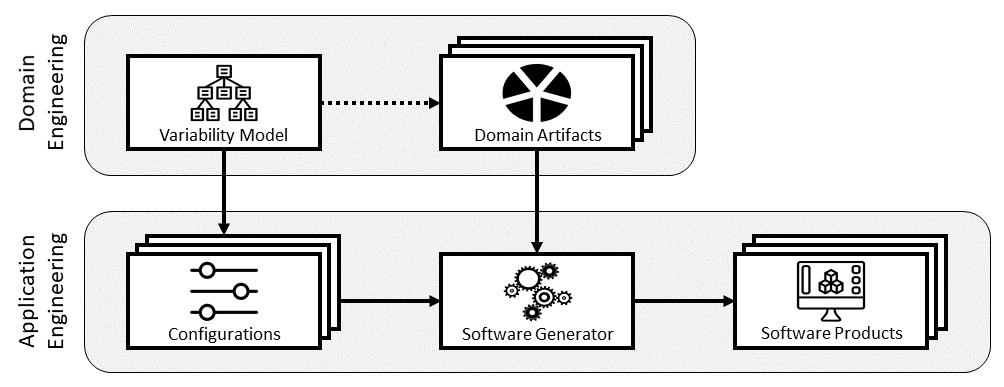
\includegraphics[width=\textwidth]{images/SPL}
    \caption{Generierung von Software-Produktlinien nach \cite{Thuem2014}\label{fig:spl}}
\end{figure}

Die in dieser Arbeit betrachtete Implementierungstechnik von Features basiert auf Anweisungen beziehungsweise Bedingungsdirektiven des C-Präprozessors. Die für diese Arbeit relevanten Direktiven lauten \texttt{\#IFDEF} und \texttt{\#IFNDEF}. Einfache Beispieleinsätze für beide Direktiven sind in \autoref{example1} und \autoref{example2} zu sehen. Sie wurden jeweils aus der wissenschaftlichen Literatur entnommen \cite{Medeiros2018,Preschern2019}. Die Direktive \texttt{\#IFDEF} leitet in \autoref{example1} den Code des Features \texttt{\_\_unix\_\_} ein, welcher mit der Anweisung \texttt{\#ENDIF} endet. Der in den Zeilen 2 bis 6 angegebene Codeteil wird genau dann ausgeführt, wenn das Feature \texttt{\_\_unix\_\_} im Rahmen der Konfiguration des Softwareproduktes definiert beziehungsweise aktiviert ist \cite{Stallmann2016}. In diesem Fall wird die Bedingung der Direktive erfolgreich erfüllt \cite{Stallmann2016}. Sie schlägt fehl, wenn das Feature nicht definiert beziehungsweise nicht aktiviert ist \cite{Stallmann2016}. Die Direktive \texttt{\#IFNDEF} wird für Code verwendet, der ausgeführt werden soll, wenn ein Feature nicht definiert ist. Im Falle des Beispiels in \autoref{example2} wird der in Zeile 3 angedeutete Code nur ausgeführt, wenn \texttt{NO\_XMALLOC} nicht aktiviert wurde.
Es besteht zudem die Möglichkeit, Features bzw. ihren Code zu verschachteln. Ein Beispiel dafür ist in \autoref{example3} angegeben. Es ist zu erkennen, dass sich der Code von \texttt{FEAT\_MZSCHEME} innerhalb des bedingten Codes von \texttt{USE\_XSMP} befindet. Der in Zeile 5 angedeutete Code kann somit nur ausgeführt werden, wenn \texttt{USE\_XSMP} aktiviert ist. Im Fall von Verschachtelung beendet ein \texttt{\#ENDIF} immer das nächstgelegene \texttt{\#IFDEF} oder \texttt{\#IFNDEF} \cite{Stallmann2016}. Es besteht zudem die Möglichkeit, Direktiven mittels \glqq und\grqq{} (\texttt{\&\&}, \texttt{and}) oder \glqq oder\grqq{} (\texttt{||}, \texttt{or}) zu erweiterten Bedingungen zu verknüpfen, die zudem Negation in Form des \texttt{!}-Operators (anstelle von \texttt{\#IFNDEF}) enthalten können \cite{Stallmann2016,Queiroz2015}. Dargestellt ist dies in \autoref{example4}.

\noindent\begin{minipage}{.45\textwidth}
\begin{lstlisting}[caption=Beispieleinsatz von \texttt{\#IFDEF} nach \cite{Preschern2019},frame=tlrb,language=C, label=example1]{example1}
#IFDEF __unix__
	#include "directorySelection.h"
	#include "directoryNames.h"
	void getDirectoryName(char* dirname) {
		getHomeDirectory(dirname);
	}
#ENDIF
\end{lstlisting}
\end{minipage}\hfill
\begin{minipage}{.45\textwidth}
\begin{lstlisting}[caption=Beispieleinsatz von \texttt{\#IFNDEF} nach \cite{Medeiros2018},frame=tlrb,language=C, label=example2]{example2}
int test = 1;
#IFNDEF NO_XMALLOC
	test = memory != NULL;
#ENDIF
if (test){
 // Lines of code here..
 } 
\end{lstlisting}
\end{minipage}

\noindent\begin{minipage}{.45\textwidth}
\begin{lstlisting}[caption=Beispiel eines verschachtelten Einsatzes von \texttt{\#IFDEF} nach \cite{Medeiros2018} ,frame=tlrb,language=C, label=example3, firstnumber=1]{example3}
bool time = msec > 0;
#IFDEF USE_XSMP
	time = time && xsmp_icefd != -1;
	#IFDEF FEAT_MZSCHEME
 		time = time || p_mzq > 0;
	#ENDIF
#ENDIF
if (time)
 gettime(&start_tv);
\end{lstlisting}
\end{minipage}\hfill
\begin{minipage}{.45\textwidth}
\begin{lstlisting}[caption=Beispiele von erweiterten Bedingungen nach \cite{Queiroz2015},frame=tlrb,language=C, label=example4, firstnumber=1]{example4}
#IFDEF FEATURE_A && FEATURE_B
	(...)
#ENDIF
(...)
#IFDEF !FEATURE_A && FEATURE_C
	(...)
#ENDIF
\end{lstlisting}
\end{minipage}

Die in den Listings gezeigten Beispiele zeigen jeweils nur den Featurecode in einer Methode beziehungsweise in einer Datei. Fragmente des Featurecodes erstrecken sich jedoch nicht nur möglicherweise mehrfach über eine Datei, sondern über mehrere Dateien - der Featurecode ist somit verstreut (englisch: code scattering), um eine Funktionalität des Features in der Gesamtheit der Software zu ermöglichen. Ein Defekt innerhalb eines Fragmentes des Featurecodes kann allerdings dazu führen, dass die gesamte Funktionalität des Features beeinträchtigt oder unterbunden wird, da der Fehler übergreifend wirkt (englisch: cross-cutting). Ebenfalls kann ein solcher Fehler dazu führen, dass die Funktionalität des gesamten Sourcecodes beeinträchtigt wird.

\section{Machine-Learning-Klassifikation}
\label{classification}

Das Themengebiet des Machine Learnings (ML) ist in zwei Teilgebiete unterteilt - das unüberwachte ML (englisch: unsupervised ML) und das überwachte ML (englisch: supervised ML). Die Methoden in diesen Teilgebieten verfolgen unterschiedliche Ziele. Im Rahmen des unüberwachten ML werden Prozesse durchgeführt, welche dazu dienen, die Struktur einer unbekannten Eingabemenge an Daten zu erlernen und anschließend zu repräsentieren \cite{Sammut2017}. Eine gängige Anwendung des unüberwachten ML ist das Clustering. Das überwachte ML beschreibt wiederum einen Prozess, welcher beabsichtigt, Vorhersagen über unbekannte Eingabedaten auf Basis des Trainings einer Abbildungsfunktion zu treffen \cite{Sammut2017}. Die Attribute \glqq unüberwacht\grqq{} und \glqq überwacht\grqq{} erhalten die Methoden aufgrund ihrer Art des Lernens beziehungsweise des Trainings. In der Anwendung des unüberwachten ML werden die Eingabedaten erfasst, gegebenenfalls vorverarbeitet, um dann auf deren Basis ein Modell zu erlernen, welches die Darstellung beziehungsweise Repräsentation der Eingabedaten bestimmt \cite{Alpaydin2010}. Auf der anderen Seite wird unter Anwendung des überwachten ML ein Modell auf Basis eines sogenannten \glqq gelabelten\grqq{} (beschrifteten) Datensatzes durch Merkmalsextraktion in Form von Attributen und dem Training auf der Grundlage der extrahierten Merkmale erstellt \cite{Alpaydin2010}. Der Datensatz, welcher zum Training verwendet wird, wird im gängigen Sprachgebrauch des Machine Learning Datenset (englisch: dataset) genannt. Das aus dem Training resultierende Modell wird Klassifikator (englisch: classifier) genannt. Gängige Anwendungen des überwachten ML sind Regression und Klassifikation. In dieser Arbeit kommt die Klassifikation als Anwendung des überwachten ML zum Einsatz. Der grundlegende Prozess der Machine-Learning-Klassifikation ist in \autoref{fig:ml} anhand eines Beispiels dargestellt.

\begin{figure}[ht]
    \centering
    \captionsetup{justification=centering,margin=2cm}
    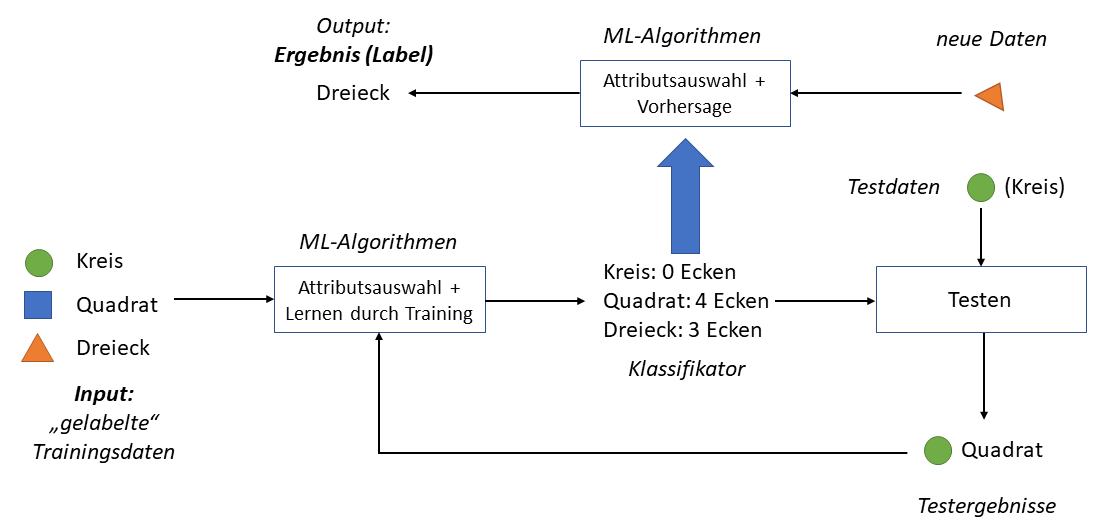
\includegraphics[width=\textwidth]{images/ML}
    \caption{Allgemeiner Prozess des überwachten Machine Learnings dargestellt anhand eines Beispiels (vereinfacht)}\label{fig:ml}
\end{figure}

Die Abbildung zeigt den Prozess des überwachten Machine Learnings anhand des Beispiels des Trainings eines Klassifikators zur Erkennung beziehungsweise Vorhersage von geometrischen Formen. Der Prozess beginnt mit den \glqq gelabelten\grqq{} Eingabedaten (A). Die Werte der Label (kategorial oder numerisch) stellen dabei die zu vorhersagende Zielklasse dar. In diesem Falle bilden die Namen der geometrischen Formen die Label als kategorischen Wert. Die Rohdaten der Eingabemenge bestehen aus den geometrischen Formen selbst. Beide Datenmengen bilden das Datenset. Um nun einen Klassifikator trainieren zu können, müssen Merkmale der Eingangsdaten ausgewählt werden, anhand derer diese identifiziert werden können (B). Diese zu identifizierenden Charakteristika der Daten werden Attribute genannt. Diese Attribute können bereits vor dem Training festgelegt werden oder automatisiert extrahiert werden. Im vorliegenden Fall wurde die Metrik \glqq Anzahl der Ecken der geometrischen Formen\grqq{} als Attribut zum Training ausgewählt. Das Ergebnis ist der fertig trainierte Klassifikator, welcher das antrainierte Wissen auf neue Daten abbilden kann (C). Ein Teil des Datensets wird in der Regel verwendet, um den Klassifikator nach dessen Erstellung zu testen (D). Die in der Regel verwendeten Verhältnisse (englisch: Split-Ratio) zwischen Trainings- und Testdaten betragen $80:20$ (basierend auf dem Paretoprinzip) oder $75:25$ (zum Beispiel \cite{Queiroz2016}). Diese Testdaten werden dem Klassifikator als Eingabemenge zur Klassifikation ohne Label zur Verfügung gestellt. Die Label sollten jedoch nicht verworfen werden, da sie als Vergleichsgrundlage für die Vorhersageperformanz des Klassifikators dienen. Sie bilden die sogenannte \glqq Ground Truth\grqq{} (deutsch: Grundwahrheit). Dazu werden die vom Klassifikator vorhergesagten Label mit denen der Ground Truth verglichen. Sollte dieser Vergleich ergeben, dass die Label große Abweichungen zeigen, so kann der Klassifikator erneut mit anderen Attributen oder einer veränderten Split-Ratio trainiert werden. Erfüllt der Klassifikator die Anforderungen an die Performanz der Vorhersagen, so ist dieser bereit, Vorhersagen auf Basis neuer Eingabedaten zu treffen (E). Dazu müssen von den neuen Daten die Attribute ermittelt werden. Auf Basis dieser trifft der Klassifikator die Vorhersage und liefert als Ausgabe das Label des Wertes der Zielklasse. Im Voraus des Testens mit den Testdaten (D) werden in manchen Fällen zudem sogenannte Validierungsdaten verwendet. Dabei handelt es sich um eine eigenständige Teilmenge der Trainingsdaten, welche verwendet wird, um die Klassifikatoren nach jedem Training zu evaluieren, um die Auswahl der Attribute hinsichtlich der Performanz auf Eignung zu prüfen \cite{Sammut2017}. Die Anwendung der Testdaten erfolgt dann im Anschluss.

Der in \autoref{fig:ml} dargestellte Klassifikator stellt einen multinomiellen oder multi-class Klassifikator dar, da er zu drei oder mehr Werten der Zielklasse zuordnen kann \cite{Sammut2017}. Für viele praktische Anwendungen genügt jedoch ein binärer Klassifikator, welcher Vorhersagen zu zwei Werten der Zielklasse trifft. Dies trifft auch auf die Klassifikatoren dieser Arbeit zu.

Nachfolgend wird eine Auswahl an Klassifikationsalgorithmen vorgestellt. Diese zählen zu den meist verwendeten Algorithmen und finden auch in dieser Arbeit ihre Anwendung.

\label{algorithms}
\textbf{Decision Trees\medskip}\\
Decision Trees (deutsch: Entscheidungsbäume) zählen zu den meistverwendeten Klassifikatoren im Bereich des supervised Machine Learnings. Studien belegen, dass sie hinsichtlich der Verwendung im Kontext der Fehlererkennung die häufigste Anwendung finden \cite{Son2019}. Decision Trees sind gerichtete und verwurzelte Bäume, die als rekursive Partition der Eingabemenge des Datensets aufgebaut werden \cite{Rokach2005}. Den Ursprung des Baumes bildet die Wurzel, welche keine eingehenden Kanten besitzt - alle weiteren Knoten besitzen jedoch eine eingehende Kante \cite{Rokach2005}. Diese Knoten teilen wiederum die Eingabemenge anhand einer vorgegebenen Funktion in zwei oder mehr Unterräume der Menge auf \cite{Rokach2005}. Meist geschieht dies anhand eines Attributs, sodass die Eingabemenge anhand der Werte des einzelnen Attributs geteilt wird \cite{Rokach2005}. Die Blätter des Baumes bilden die Zielklassen ab. Eine Klassifizierung kann folglich durchgeführt werden, indem man von der Wurzel bis zu einem Blatt den Kanten anhand der entsprechenden Werte der Eingangsmenge folgt. Es existieren verschiedene Algorithmen zur Erstellung von Decision Trees. Bekannte Stellvertreter dieser sind ID3, C4.5 (J48) und CART \cite{Rokach2005}. Der grundlegende Aufbau eines Decision Trees ist in \autoref{fig:dt} dargestellt.

\begin{figure}[ht]
    \centering
    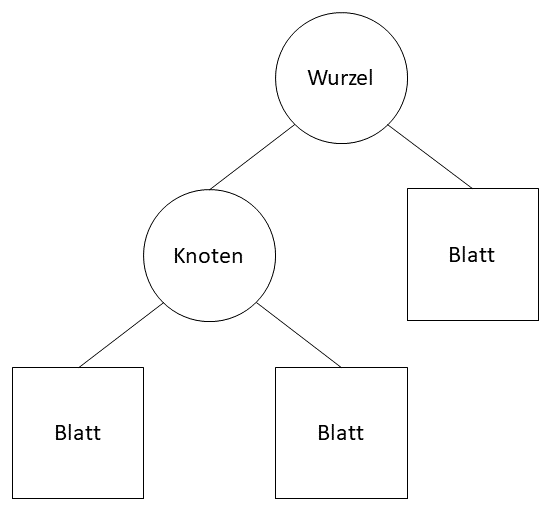
\includegraphics[width=0.5\textwidth]{images/DT}
    \caption{Grundsätzlicher Aufbau eines Decision Trees\label{fig:dt}}
\end{figure}

Eine Besonderheit von Decision Trees stellen sogenannte Random Forests dar. Diese beschreiben eine Menge von Klassifikatoren, bei der mehrere einzelne Decision Trees gleichzeitig erzeugt werden und deren Ergebnisse anschließend aggregiert werden \cite{Alam2013}. Dazu erhält jeder Decision Tree eine Teilmenge der Eingabemenge des Datensets \cite{Alam2013}. Random Forests eigenen sich besonders zur Anwendung, wenn viele Attribute im Datenset vorhanden sind \cite{Alam2013}.

\textbf{k-Nearest-Neighbors\medskip}\\
Ein k-Nearest-Neighbor-Klassifikator (deutsch: k-nächste-Nachbarn) basiert auf zwei Konzepten \cite{Zhang2016}. Das erste Konzept basiert auf der Abstandsmessung zwischen den Werten der zu klassifizierenden Datenmenge und den Werten der Attribute des Datensets \cite{Zhang2016}. Die Abstandmessung erfolgt in der Regel durch die Berechnung der Euklidischen Distanz $D(p,q)$:

\[D(p,q) = \sqrt{\sum_1^n(p_{n}-q_{n})^{2}}\] 

Die Anzahl der Attribute wird durch den Parameter $n$ wiedergegeben, $p$ und $q$ repräsentieren jeweils die Werte der zu klassifizierenden Datenmenge und die Werte der Attribute des Datensets. Das zweite Konzept bildet der Parameter $k$, der angibt, wie viele nächste Nachbarn zum Vergleich der zuvor berechneten Abstände in Betracht gezogen werden \cite{Zhang2016}. Bei einem $k > 1$ wird diejenige Zielklasse gewählt, deren Auftreten innerhalb der nächsten Nachbarn überwiegt.

\textbf{Künstliche neuronale Netze\medskip}\\
Künstliche neuronale Netze (KNN, englisch: Artificial Neural Networks) verwenden nicht-lineare Funktionen zur schrittweisen Erzeugung von Beziehungen zwischen der Eingabemenge und den Zielklassen durch einen Lernprozess \cite{Linder2004}. Sie sind angelehnt an die Funktionsweise von biologischen Nervensystemen und bestehen aus einer Vielzahl von verbundenen Berechnungsknoten, den Neuronen \cite{OShea2015}. Der grundsätzliche Aufbau eines künstlichen neuronalen Netzes kann in \autoref{fig:ann} eingesehen werden. Der Lernprozess besteht aus zwei Phasen - einer Trainingphase und einer Recall-Phase \cite{Linder2004}. In der Trainingsphase werden die Eingabedaten, meist als multidimensionaler Vektor, in den Input-Layer geladen und anschließend an die Hidden-Layer verteilt \cite{OShea2015}. In den Hidden-Layers werden dann Entscheidungen anhand der Beziehungen zwischen den Eingabedaten und Zielklassen sowie die den Verbindungen zuvor zugewiesenen Gewichtsfaktoren getroffen \cite{Linder2004,OShea2015}. Im Rahmen der Recall-Phase wird die Vorhersage basierend auf der zu klassifizierenden Datenmenge anhand der zuvor getroffenen Entscheidungen der Hidden-Layers getroffen und an die jeweiligen Output-Layer, welche die Werte der Zielklasse repräsentieren, weitergeleitet \cite{Linder2004}. 

\begin{figure}[ht]
    \centering
    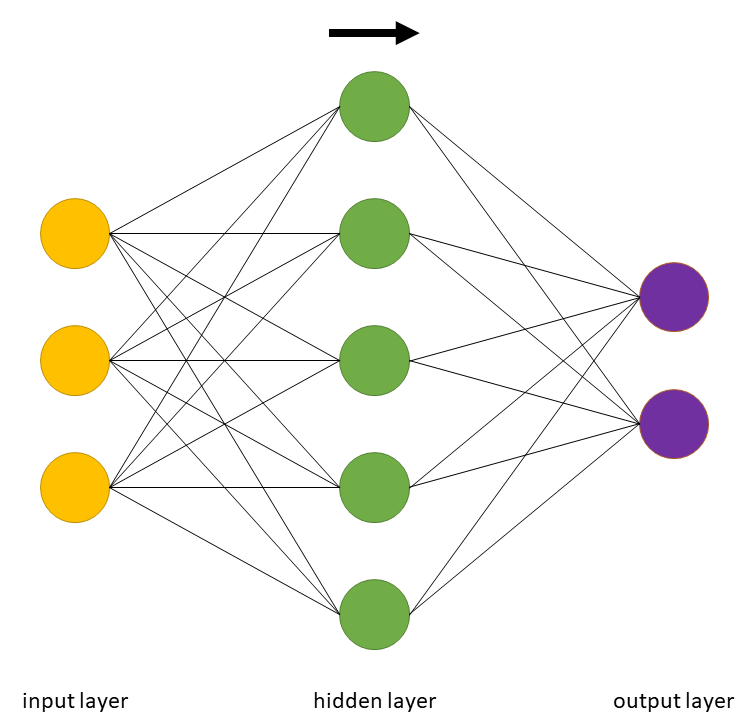
\includegraphics[width=0.5\textwidth]{images/ANN}
    \caption{Grundsätzlicher Aufbau eines KNN mit drei Input-Layer-Neuronen, fünf Hidden-Layer-Neuronen und zwei Output-Layer-Neuronen\label{fig:ann}}
\end{figure}

\textbf{Logistische Regression\medskip}\\
Logistische-Regressions-Klassifikatoren (englisch: Logistic Regression) basieren auf dem mathematischen Konzept des Logits, welcher den natürlichen Logarithmus eines Chancenverhältnisses beschreibt \cite{Peng2002}. Seine Formel lautet:

\[logit(Y) = ln(\frac{\pi}{1-\pi})\]

$Y$ beschreibt dabei die zu klassifizierende Datenmenge, wohingegen $\pi$ die Verhältnisse der Wahrscheinlichkeiten der Werte der Attribute der Eingabemenge bezeichnet. Am besten geeignet ist dieser Klassifikator für eine Kombination aus kategorialen oder numerischen Eingabedaten und kategorischen Zielklassen \cite{Peng2002}.

\textbf{Na\"{\i}ve Bayes\medskip}\\
Na\"{\i}ve-Bayes-Klassifikatoren zählen zu den linearen Klassifikatoren und basieren auf dem Satz von Bayes. Die Bezeichnung \glqq naiv\grqq{} erhält der Klassifikator durch die Annahme, dass die Attribute der Eingabemenge unabhängig voneinander sind \cite{Raschka2014}. Diese Annahme wird zwar in der realen Verwendung des Klassifikators häufig verletzt, dennoch erzielt er in der Regel eine hohe Performanz \cite{Raschka2014}. Der Klassifikator gilt als effizient, robust, schnell und einfach implementierbar \cite{Raschka2014}. Die zur Durchführung einer Klassifikation mittels Na\"{\i}ve Bayes benötigte Formel nach Thomas Bayes ist in \autoref{fig:nb} samt Erläuterung der einzelnen Faktoren aufgeführt.

\begin{figure}[ht]
    \centering
    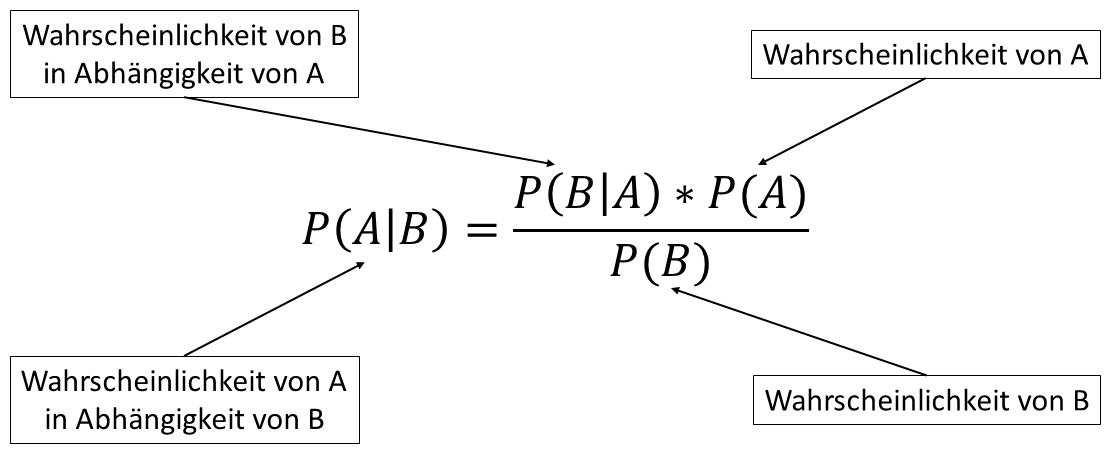
\includegraphics[width=0.6\textwidth]{images/NB}
    \caption{Satz von Bayes als Grundlage des Na\"{\i}ve-Bayes-Klassifikators\label{fig:nb}}
\end{figure}

Es existiert zudem eine Mehrzahl an Varianten des Na\"{\i}ve-Bayes-Klassifikators, die verschiedene Annahmen über die Verteilung der Attribute der Eingabemenge machen. Beispiele dafür sind der Gaußsche-Na\"{\i}ve-Bayes (normalverteilte Attribute), der multinomiale Na\"{\i}ve-Bayes (multinomiale Verteilung der Attribute) sowie der Bernoulli-Na\"{\i}ve-Bayes (unabhängige binäre Attribute).

\textbf{Stochastic Gradient Descent\medskip}\\
Ein Stochastic-Gradient-Descent-Klassifikator basiert auf dem Gradientenverfahren (englisch: Gradient Descent), welches das Ziel hat, mittels einer Kostenfunktion $f$ zu einem gegebenen $x$ das minimale $y$ zu finden \cite{Srinivasan2019}. Im Falle der Klassifikation mittels Machine Learning bedeutet dies, dass die Funktion $f$ auf Basis der Trainingsdaten erzeugt wird, die wiederum die Attribute der Daten auf die Werte der Zielklasse überträgt \cite{Diab2019}. Eine festgelegte Kostenfunktion, versucht dann auf Basis der Trainingsdaten ($x$) die minimale Fehlerquote für die Vorhersagen ($y$) anhand von verschiedenen Koeffizientenwerten zu ermitteln \cite{Diab2019}.

\textbf{Support Vector Machines\medskip}\\
Support Vector Machines verfolgen das Ziel, eine sogenannte \glqq Hyperplane\grqq{} in einem $n$-dimen-sionalen Raum ($n$ = Anzahl der Attribute der Eingabemenge) zu finden, welche die Datenpunkte der Eingabemenge eindeutig klassifizieren kann \cite{Gandhi2018}. Die Hyperplane beschreibt eine Trennlinie beziehungsweise Trennfläche, mit deren Hilfe die Daten der zu klassifizierenden Menge den Zielklassen zugeordnet werden können \cite{Luber2019}. Dabei gilt es, dass die Trennflächen, welche die Eingangsmenge anhand der Attribute in verschiedene Trennungsebenen unterteilen, einen möglichst großen Abstand ohne Datenpunkte voneinander haben \cite{Luber2019}. Dies funktioniert sowohl für linear als auch nicht-lineare trennbare Mengen.

\section{Fehlervorhersage mittels Machine Learning}

Der Hintergrund der Fehlervorhersage mittels Machine Learning basiert auf dem zuvor vorgestellten Konzept des überwachten Machine Learnings. Als Grundlage dienen dabei meist Daten, die aus Software-Repositories entnommen beziehungsweise extrahiert werden. Viele Studien und wissenschaftliche Arbeiten setzen jedoch auch auf vorgefertigte Datensets, wie zum Beispiel von der NASA oder von Eclipse \cite{Son2019}. Die zugehörigen Label der Datensets lauten in der Regel \glqq fehlerfrei\grqq{} und \glqq defekt\grqq{} und können auf verschiedene Weisen ermittelt werden. Eine gängige Methode ist die Identifizierung von korrektiven und fehlereinführenden Commits als Entscheidungsgrundlage für das Label. Die üblichen Vorgehensweisen setzen auf die Einbindung von Bugtracking-Systemen oder die Analyse von Commit-Nachrichten zur Identifizierung der korrektiven Commits \cite{Queiroz2016,Zimmermann2007}. Fehlereinführende Commits können anschließend unter Verwendung von Git-Kommandos oder durch die Anwendung des sogenannten SZZ-Algorithmus ermittelt werden. Dieser Algorithmus wird in dieser Arbeit verwendet und in \hyperref[szz-def]{Abschnitt 3.2} erläutert. Auf Basis dieser Daten werden die Attribute bestimmt. Dabei handelt es sich in der Regel um Metriken, die entweder die Charakteristika des Sourcecodes (Codemetriken) oder Aktivitäten und Prozesse im Bezug auf Software-Repositories (Prozessmetriken) beschreiben \cite{Son2019,Rahman2013}. Mithilfe dieser Attribute werden die Klassifikatoren trainiert. Eine Studie, welche 156 wissenschaftliche Arbeiten zum Thema der Fehlervorhersage mittels Machine Learning analysierte, ergab, dass besonders Entscheidungsbaum-basierte, Bayessche Verfahren, Regression und künstliche neuronale Netze als Klassifikationsalgorithmen zur Anwendung kommen \cite{Son2019}. Diese Algorithmen wurden unter anderem auch in dieser Arbeit verwendet. Erläuterungen können in \hyperref[algorithms]{Abschnitt 4.1} gefunden werden. Die fertig trainierten Klassifikatoren können dann auf Basis neuer Daten Vorhersagen zum Zustand einer Software treffen. Die Vorhersagen beruhen in der Regel auf defekten Dateien im Kontext von Commits oder Releases.

Als Beispiel für zwei konkrete Anwendungen von Machine Learning gestützter Fehlervorhersage werden im Folgenden zwei wissenschaftliche Arbeiten vorgestellt. Die erste Arbeit \glqq Comparative Analysis of the Efficiency of Change Metrics and Static Code Attributes for Defect Prediction\grqq{} von Moser et al. \cite{Moser2008} stellt eine Methodik zur dateibasierten Fehlervorhersage vor. Die zweite Arbeit \glqq Towards Predicting Feature Defects in Software Product Lines\grqq{} von Queiroz et al. \cite{Queiroz2016} knüpft an den zuvor vorgestellten Ansatz der Software-Features an. Beide Literaturquellen werden im weiteren Verlauf dieser Arbeit eine Rolle spielen, die im jeweiligen Abschnitt erläutert werden.

\subsection*{Dateibasierte Fehlervorhersage}
\label{moser}

Das Beispiel zur dateibasierten Fehlervorhersage stammt aus einer wissenschaftlichen Arbeit von Moser et al. \cite{Moser2008}. Sie widmet sich einer vergleichenden Analyse von zwei verschiedenen Mengen von Metriken zur dateibasierten Fehlervorhersage mittels Methoden des Machine Learnings. Die Zuordnung erfolgt in \glqq defekt\grqq{} und \glqq defektfrei\grqq. Als Datenbasis dient ein vorgefertigtes Datenset von Eclipse. Auf Basis dieses Datensets wurden \glqq produktbasierte\grqq{} Metriken (Codemetriken) und Prozessmetriken berechnet. Zur Anwendung kamen die Klassifikationsalgorithmen logistische Regression, Na\"{\i}ve Bayes und Entscheidungsbäume. Die Prozessmetriken stellen eine Besonderheit dieser Arbeit dar, da sie in dieser Arbeit zum ersten Mal näher betrachtet und auf ihre Eignung als Attribute zum Training der Klassifikatoren erörtert wurden. Die Metriken berechneten unter anderem die Anzahl der Änderungen an einer Datei, die Anzahl der Autoren einer Datei, die Anzahl der hinzugefügten oder entfernten Zeilen einer Datei oder das Alter einer Datei. Das Resultat der Arbeit lautet, dass Prozessmetriken effektiver zur Fehlervorhersage genutzt werden können als Codemetriken. Im Folgenden werden die 17 Prozessmetriken samt ihrer Beschreibungen und Abkürzungen (für diese Arbeit) vorgestellt.

\label{moser-metrics}
\begin{multicols}{2}
\begin{itemize}
\setlength{\itemsep}{-2pt}
\item REVISIONS (REVI)\\Anzahl der Revisionen (Bearbeitungen) der Datei.
\item REFACTORINGS (REFA)\\Anzahl der Fälle, in denen die Datei in einem Refactoring involviert war. Basierend auf Analyse der Commit-Nachricht auf das Vorhandensein des Begriffs "refactor".
\item BUGFIXES (BUGF)\\Anzahl der Fälle, in denen die Datei in einer Fehlerbehebung involviert war.
\item AUTHORS (AUTH)\\Anzahl der verschiedenen Autoren, die die Datei in das Repository eingecheckt haben.
\item LOC\_ADDED (ADDL)\\Summe der zur Datei hinzugefügten Codezeilen über alle Revisionen.
\item MAX\_LOC\_ADDED (ADDM)\\maximale Anzahl von Codezeilen, die für alle Revisionen hinzugefügt wurden.
\item AVE\_LOC\_ADDED (ADDA)\\durchschnittlich hinzugefügte Codezeilen pro Revision.
\item LOC\_DELETED (REML)\\Summe der von der Datei entfernten Codezeilen über alle Revisionen.
\item MAX\_LOC\_DELETED (REMM)\\maximale Anzahl von Codezeilen, die für alle Revisionen entfernt wurden.
\item AVE\_LOC\_DELETED (REMA)\\durchschnittlich entfernte Codezeilen pro Revision.
\item CODECHURN (CCHN)\\Summe von (hinzugefügte Codezeilen - entfernte Codezeilen) über alle Revisionen.
\item MAX\_CODECHURN (CCHM)\\maximaler CODECHURN für alle Revisionen.
\item AVE\_CODECHURN (CCHA)\\durchschnittlicher CODECHURN pro Revision.
\item MAX\_CHANGESET (MAXC)\\maximale Anzahl von Dateien, die gemeinsam committed wurden.
\item AVE\_CHANGESET (AVGC)\\durchschnittliche Anzahl von Dateien, die gemeinsam committed wurden.
\item AGE (AAGE)\\Alter der Datei in Wochen (rückwärts zählend bis zu einem bestimmten Release).
\item WEIGHTED\_AGE (WAGE)\\$\text{Weighted Age} = \frac{\sum_{i=1}^N Age(i)*LOC\_ADDED(i)}{\sum_{i=1}^N LOC\_ADDED(i)}$
\end{itemize}
\end{multicols}

Im Rahmen der Evaluation (\hyperref[classic-eval]{Abschnitt 5.2}) dienen diese dateibasierten Metriken als Grundlage für den Vergleich, ob die Metriken des für diese Arbeit erstellten featurebasierten Datensets einen Einfluss auf die Ergebnisse der Fehlervorhersage auf Dateiebene hervorrufen. 

\subsection*{Featurebasierte Fehlervorhersage}

Das Beispiel zur featurebasierten Fehlervorhersage stammt aus einer wissenschaftlichen Arbeit von Queiroz et al. \cite{Queiroz2016}. Bei dieser Fallstudie handelt es sich um die erste und bisher einzige Arbeit über Fehlervorhersage mit Bezug zu Software-Features. Sie stellt somit für diese Masterarbeit eine bedeutende literarische Grundlage dar. Der Ablauf des von Queiroz et al. angewandten Prozesses zur Erstellung eines featurebasierten Datensets und dessen Anwendung zum Training von Klassifikatoren orientiert sich am zuvor vorgestellten allgemeinen Prozess des überwachten Machine Learnings.

Die Erläuterung des Beispiels erfolgt anhand von zwei Abbildungen, welche den in der Arbeit von Queiroz et al. vorgestellten Prozess in zwei Teilen visualisieren. Der erste Teil ist in \autoref{fig:ml1} dargestellt.

\begin{figure}[ht]
    \centering
    \captionsetup{justification=centering}
    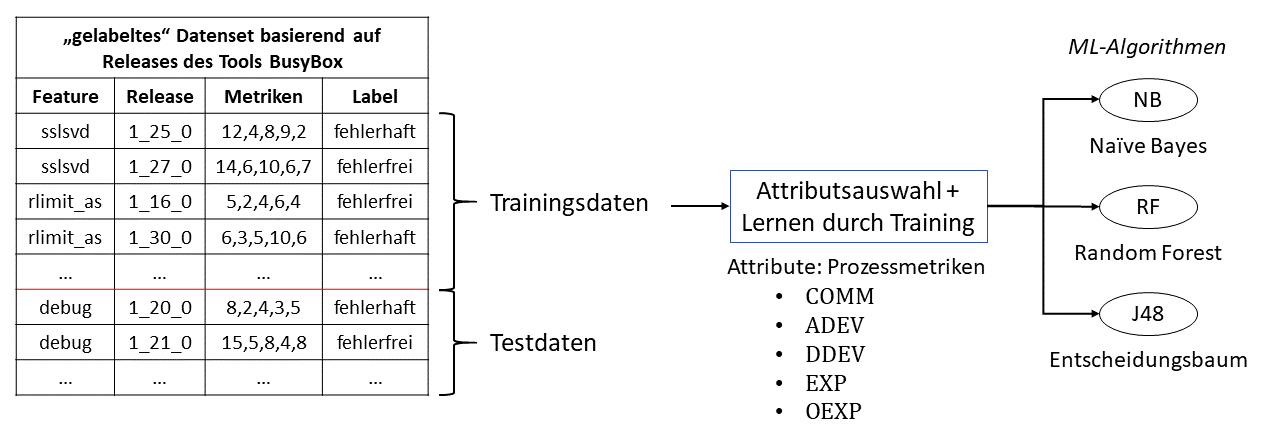
\includegraphics[width=\textwidth]{images/ML1}
    \caption{Teil 1: Featurebasierter Prozess des überwachten Machine Learnings nach \cite{Queiroz2016}}\label{fig:ml1}
\end{figure}

\subsubsection*{Datenset}

Die Datenbasis des Datensets bilden historische Commits des UNIX-Toolkits BusyBox\footnote{\url{https://busybox.net/}}, dessen Quellcode frei verfügbar in einem Git-Repository\footnote{\url{https://git.busybox.net/busybox/}} eingesehen und von dort geklont werden kann. Diese Commits wurden wiederum ihren entsprechenden Releases zugeordnet, welche auf der vergebenen Tag-Struktur des Repositories beruhen. Ferner wurden aus den Diffs der Commits die dort bearbeiteten Features extrahiert und anschließend zusammen mit den Release-Informationen in einer MySQL-Datenbank gespeichert. Zusätzlich enthält jeder Datenbankeintrag aggregierte Werte von fünf auf das Feature und den Release bezogenen Prozessmetriken (Erläuterung folgt) sowie das binäre Label, ob ein Feature in einem Release fehlerhaft oder fehlerfrei war. Ein Feature gilt in einem Release als fehlerhaft, sofern in einem Commit des darauffolgenden Releases ein fehlerbehebender Commit bezüglich des Features festgestellt werden konnte. Dies geschieht über die Analyse der Commit-Nachrichten. Sofern eine Commit-Nachricht die Begriffe \glqq bug\grqq{} (Fehler), \glqq error\grqq{} (schwerwiegender Fehler), \glqq fail\grqq{} (fehlschlagen) oder \glqq fix\grqq{} (beheben) enthält, werten die Autoren des Papers den Commit als fehlerbehebend. Alternative Methoden zur Durchführung dieser Analyse bestehen aus der Einbindung von Daten aus Bug-Tracking-Systemen, die häufig an Software-Repositories angebunden sind, sowie aus der Anwendung des sogenannten SZZ-Algorithmus, welcher in dieser Arbeit verwendet wurde und in \hyperref[szz-def]{Abschnitt 3.2} erläutert wird \cite{Sliwerski2005,Zimmermann2007}. Wie im Rahmen des überwachten Machine Learning üblich, wird das Datenset in Trainings- und Testdaten in einem Verhältnis von $75:25$ geteilt. 

\subsubsection*{Metriken und Klassifikation}

Die Trainingsdaten werden dann den Klassifikatoren zum Training zur Verfügung gestellt. Als Attribute dienen fünf Prozessmetriken mit spezifischer Betrachtung von Software-Features. Einen Überblick über die Beschreibungen dieser gibt \autoref{tab:metrics-rodrigo}. Diese Metriken werden auch für diese Arbeit im Rahmen der Erstellung des featurebasierten Datensets übernommen. Als Klassifikationsalgorithmen wurden Na\"{\i}ve Bayes, Random Forest und J48-Entscheidungsbäume gewählt.

\begin{table}[ht]
\centering
\caption{Übersicht der von \cite{Queiroz2016} verwendeten Prozessmetriken}
\label{tab:metrics-rodrigo}
\begin{tabular}{|c|l|} 
\hline
\textbf{Metrik}  & \textbf{Beschreibung}  \\ 
\hline
COMM & \begin{tabular}[c]{@{}l@{}}Anzahl der Commits, die in einem Release dem betreffenden \\ Feature gewidmet sind. \end{tabular} \\ 
\hline
ADEV & \begin{tabular}[c]{@{}l@{}}Anzahl der Entwickler, die das betreffende Feature\\in einem Release bearbeitet haben. \end{tabular} \\ 
\hline
DDEV & \begin{tabular}[c]{@{}l@{}}kummulierte Anzahl der Entwickler, die das betreffende Feature\\in einem Release bearbeitet haben. \end{tabular} \\ 
\hline
EXP & \begin{tabular}[c]{@{}l@{}}geometrisches Mittel der \glqq Erfahrung*\grqq{} aller Entwickler, die am \\ betreffenden Feature in einem Release gearbeitet haben. \end{tabular} \\ 
\hline
OEXP & \begin{tabular}[c]{@{}l@{}}\glqq Erfahrung*\grqq{} des Entwicklers, der am meisten zum betreffenden \\ Feature in einem Release beigetragen hat. \end{tabular} \\ 
\hline
\multicolumn{2}{|c|}{\begin{tabular}[c]{@{}c@{}}*Erfahrung ist definiert als Summe der geänderten, gelöschten\\oder hinzugefügten Zeilen im zugehörigen Release. \end{tabular}} \\
\hline
\end{tabular}
\end{table}

\begin{figure}[ht]
    \centering
    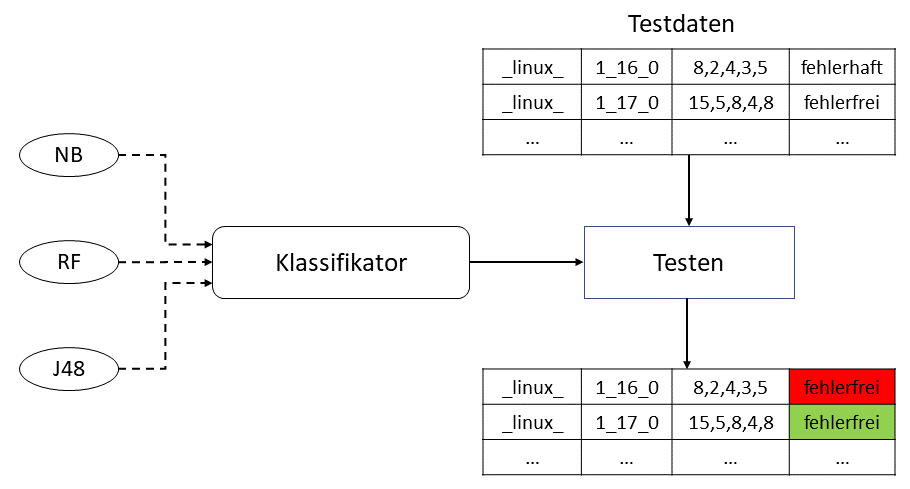
\includegraphics[width=0.8\textwidth]{images/ML2}
    \caption{Teil 2: Featurebasierter Prozess des überwachten Machine Learnings nach \cite{Queiroz2016}}\label{fig:ml2}
\end{figure}

\subsubsection*{Test der Klassifikatoren}

Wie in \autoref{fig:ml2} dargestellt ist, wird für jeden Klassifikationsalgorithmus ein Klassifikator erstellt, welcher anschließend getestet und evaluiert wird. Dazu werden die jeweiligen Klassifikatoren auf das Testdatenset angewendet, ohne jedoch die Werte der Zielklassen mit anzugeben. Diese werden im Anschluss an den Klassifikationsvorgang mit den vorhergesagten Werten auf Übereinstimmung verglichen. Anhand dieses Vergleiches können die Genauigkeit sowie weitere Metriken zur Bewertung der Leistung der Klassifikatoren gemessen werden. Eine Übersicht von Evaluationsmetriken kann in \hyperref[eval-metrics]{Abschnitt 5.2.1} gefunden werden.

Die so erstellten Klassifikatoren können dann zur Vorhersage von neuen und unbekannten Daten genutzt werden, um defekte Features eines zukünftigen Releases zu identifizieren. Dazu müssen die fünf zuvor genannten Prozessmetriken dieser Daten berechnet werden. 

\cleardoublepage
